
\section{Time series model}
\label{sec:model:TSMS}

Following current database models, a \acro{TSMS} model consists of two
components: a data model and a set of operations. Measures and time
series are the main objects of our \acro{TSMS} model. 
%
In this section we describe and formalise the \acro{TSMS} model. 


\subsection{Data model}

Roughly speaking a \emph{time series} is a set of observations
collected at specific time instants. An observation may consist of
single value or multiple values collected at the same time instant.
Each pair of time and observed values is referred to as a
\emph{measure}. Then, a time series is a correspondence between times
and values. A time series can be described by a set of measures.

We name \emph{time domain} the set $\cal{T}$ of all the possible time
values. $\cal{T}$ can be either a finite or an infinite set and
usually it is a closed set. Although time is a complex issue
\cite{iep:time-supplement}, in this paper we will assume that the
$\cal{T}$ is the set of affinely extended real numbers $\Rb = \R \cup
\{+\infty,-\infty\}$. This avoids the complex details of time
modelling while being powerful enough for our purposes. Next, we
define the main time related concepts using this naive approximation.



\begin{definition}[Time concepts]
  \label{def:model:temps}
  Let $\cal{T}=\Rb$ be the domain for time.
  %
  We name an element $t\in\cal{T}$ as \emph{time instant}.
  %
  Let $s,t\in\cal{T}$ be two time instants.  We define the
  \emph{duration of time} between $s$ and $t$ as the value $d
  \in\cal{T}$ which measures the distance in time units between the
  two time instants, that is $d =|s-t|$.
\end{definition}

The value is an attribute that indicates the magnitude of a
measure. The domain for the values can be any data type. Valid domains
for values include integers, real numbers, strings, and more
elaborated data structures such as arrays, lists, or even other time
series. Here below, the domain for values will be denoted by
$\cal{V}$. 
%
Without loss of generality in this paper we will assume that the
domain of values is the set of projectively extended reals $\Rp = \R
\cup \{\infty\}$.

A measure represents an actual value measured in a particular time
instant. We define it below.

\begin{definition}[Measure]
  Let $v\in\cal{V}$ be a value and let $t\in\cal{T}$ be the time
  instant when the value was acquired. We define a \emph{measure} $m$
  as the tuple $m=(t,v)$. The domain of a measure $m$, written as
  $\dom m$, is the domain of its value.
\end{definition}

Let $m = (t,v)$ be a measure. In what follows, $V(m)$ denotes the
value $v$ and $T(m)$ denotes the time $t$.

Order between measures plays an important role. Given two measures we
define two distinct order relations.

\begin{definition}[Semitemporal order]
  Let $m$ and $n$ be two measures. We name \emph{semitemporal order}
  the binary relation written $m\leq n$, defined as $m\leq n\iff
  (T(m)<T(n) \vee m=n)$.
\end{definition}

\begin{definition}[Temporal order] Let $m$ and $n$ be two measures. We
    name \emph{temporal order} the binary relation written $m \leq^t
    n$ and defined as $m \leq^t n \iff T(m) \leq T(n)$.
\end{definition}

Note that the semitemporal order is a partial order while the temporal
order is a total order.

Intuitively speaking a time series is a ordered set of measures of the
same phenomena.  Sometimes they are also called time
sequences~\cite{last:hetland}. We define it as follows.

\begin{definition}[Time series]
  \label{def:model:timeseries}
  Let $S = \{m_0,\ldots,m_k\}\subset\cal{T}\times\cal{V}$ be a finite
  set of measures of the same type. Then, $S$ is a \emph{time series}
  iff $\forall i,j: i,j\in[0,k] \wedge i\neq j: T(m_i)\neq T(m_j)$.
  We define the domain of a time series $S$, denoted as $\dom S$, as
  the domain of its measures.
\end{definition}

Observe that although measures in $S$ are expected to be of the same
phenomena, from a formal standpoint we only require the domain of all
values to be the same. 

In a time series there are not two measures with the same time. Thus,
considering the temporal order, a time series is a totally ordered
set.

The cardinality of a time series $S=\{m_0,\dots,m_k\}$, noted as
$|S|$, is the number of measures that contains.  An empty time series is
noted as $\emptyset$. Needless to say, $|\emptyset|=0$.

Although we defined values as scalars it is easy to extend the
concept. Following~\cite{assfalg08:thesis}, a time series can record
more than one phenomena if they share the same acquisition time
instants.  This kind of series are known as \emph{multivalued time
  series}. Let $S$ be a multivalued time series and let its domain be
$\dom S={\cal{V}}_1\times\cdots\times{\cal{V}}_n$. Then, we write its
measures as $m=(t,v_1,v_2,\ldots,v_n)$.



A time series is regular when its measures are equi-spaced in time,
according to \cite{last:hetland}.  Let $S=\{m_0, m_1,\ldots,
m_{k-1},m_k\}$ be a time series, where
$T(m_0)<T(m_1)<\dots<T(m_{k-1})<T(m_k)$, and let $d\in\cal{T}$ be a
time duration. Then $S$ is \emph{regular} when $d=T(m_1)-T(m_0)=
\dots =T(m_k)-T(m_{k-1})$.




\subsection{Operations}
\label{sec:model:operations}

Time series can be manipulated through the operations defined in this
section.
%
Like the relational model operations, operations over time series
ignore the actual semantics of the data. In a particular application,
it should be decided whether an operation is semantically coherent or
must not be applied. For example, the addition of values coming from two
different phenomena could be semantically erroneous.

In this section three groups of operations are introduced, one in each
of the subsections which follow. The set operations, that consider
times series as sets; the sequence operations, that consider time
series as sequences; and the temporal operations, that manipulate the
time series assuming that are representations of functions.



\subsubsection{Set operations}
\label{sec:set}

We describe how common set operators can be applied to time series. We
rely on how the relational model of \acro{DBMS} describes operations
based on set algebra~\cite{date:introduction}.

Consider a time series $S$. $S$ is a finite ordered set (by the
temporal order). Then, if $S$ nonempty, $S$ has a maximum and a
minimum.  
%
Let $S$ be a time series. The \emph{maximum}
of $S$, denoted as $\max S$, is an element of $S$ such that $\forall m
\in S:\max S\geq^t m $.  
%
Note that $\max S$ is not defined when $S=\emptyset$. However, the
time series has a supremum even when empty. In fact, according
to~\cite{cantrell:extendedreal}, $\sup \emptyset=-\infty$.
%
Let $m=(-\infty,\infty)$ be a measure with infinite time and value.
Using this fact we define the \emph{supremum} of $S$, noted as
$\sup S$, as
\[
\sup S =\begin{cases}
  \max S    & \text{when $S$ nonempty}\\
  m   & \text{otherwise}
\end{cases}
\]
Dually, we can define the \emph{minimum} of $S$, noted as $\min S$,
and the \emph{infimum} of $S$, noted as $\inf S$.

The membership operation defines when a measure belongs to a time
series. We define two distinct membership operations. This induces two
different ways to consider time series and its operations.

Let $S$ be a time series and $m$ be a measure. 
%
We say that $m$ belongs to $S$ (plain \emph{membership}), denoted as
$m \in S$, when $\exists x\in S: x=m$.  We also say that $m$ belongs
temporally to $S$ (\emph{temporal membership}), denoted as $m \inst
S$, when $\exists x\in S : T(m)=T(x)$.


The two distinct membership criteria induce two meanings for
inclusion. Let $R$ and $S$ be two time series.  We say that $R$ is
\emph{included} in $S$, written $R\subseteq S$, when all the elements
of $R$ belong to $S$.  Analogously, we say that $R$ is \emph{included
  temporally} in $S$, noted $R\subseteqt S$, when all the elements of
$R$ belong temporally to $S$.


The \emph{union} of two sets is a set containing elements from both
sets. Usual set union operations do not apply to time series because
the result time series could have repeated time values.  Thus, we 
give a slightly modified concept for union.

The union operation requires both time series to have the same domain,
as is also true with the union operation of relational
algebra~\cite{date:introduction}.

Let $R$ and $S$ be two time series and let $\dom R =\dom S$. 
%
The \emph{union} of $R$ and $S$, noted $R\cup S$, is a new time series
$R \cup S = \{m|m\in R\vee (m\in S\wedge m \notinst R)\}$. 
%
The \emph{temporal union} of $R$ and $S$, noted $S_1 \cupt S_2$, is a
time series $R \cupt S = \{ m | (m \in R \wedge m \in S) \vee (m \in R
\wedge m \notinst S) \vee (m \in S \wedge m \notinst R) \}$.  
%
It is interesting to emphasise that the union is a non commutative
operation while the temporal union is a commutative one.

\begin{figure}
  \centering
  %\def\escala{0.9}

\def\nodeA{node [above left=0.5cm and 0.1cm] {$(1,1)$} node [below left=0.5cm and 0.1cm] {$(5,1)$}}
\def\nodeB{node [above right=0.5cm and 0.1cm] {$(2,2)$} node [below right=0.5cm and 0.1cm] {$(6,2)$}}
\def\nodeT{node [above=0.1cm] {$(4,0)$} node [left=0.4cm] {$(3,1)$} node [right=0.4cm] {$(3,2)$}}
% Definition of circles
\def\firstcircle{(0,0) circle (1.5cm)}
\def\secondcircle{(0:2cm) circle (1.5cm)}
\def\thirdcircle{(0:1cm) circle (1.11cm)}

\colorlet{circle edge}{blue!50}
\colorlet{circle area}{blue!20}

\tikzset{
  filled/.style={fill=circle area, draw=circle edge, thick},
  outline/.style={draw=circle edge, thick},
  every node/.style={transform shape}
}

%\setlength{\parskip}{5mm}






%Set A or B
\begin{tikzpicture}[scale=\escala]
  \draw[filled] \firstcircle \nodeA;
    \begin{scope}
        \clip \secondcircle;
        \draw[filled, even odd rule] \firstcircle \nodeA
                                 \secondcircle 
                                 \thirdcircle;
   \end{scope}
    \draw[outline] \firstcircle
                   \secondcircle \nodeB
                   \thirdcircle \nodeT;

   \node[anchor=south] at (current bounding box.north) {$S_1 \cup S_2$};
\end{tikzpicture}
%Set temporal A or B
\begin{tikzpicture}[scale=\escala]
    \draw[filled, even odd rule] \firstcircle \nodeA
                                 \secondcircle \nodeB
                                 \thirdcircle \nodeT;
    \node[anchor=south] at (current bounding box.north) {$S_1 \cup^t S_2$};
\end{tikzpicture}






%%% Local Variables:
%%% TeX-master: "../main"
%%% ispell-local-dictionary: "british"
%%% End:

  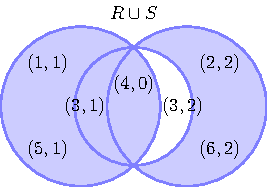
\includegraphics{fig_model_venn.pdf}
  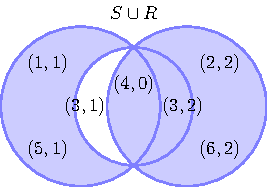
\includegraphics{fig_model_venn_reverse.pdf}
  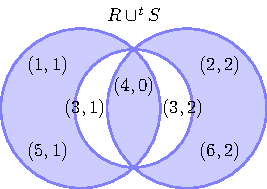
\includegraphics{fig_model_venn2.pdf}
  \caption{Venn diagrams for set and temporal set union operations of
    \acro{TSMS}}
  \label{fig:model:venn}
\end{figure}


\begin{example}\label{ex:model:s1s2}
  Let $R=\{(1,1), (3,1), (4,0), (5,1)\}$ and $S=\{(2,2), (3,2), (4,0),
  (6,2)\}$ be two time series. The union of $R$ and $S$ is $R\cup
  S=\{(1,1), (2,2), (3,1), (4,0), (5,1), (6,2)\}$. Because union is
  not symmetric, $S\cup R=\{(1,1), (2,2), \allowbreak(3,2), (4, 0), (5,1),
  (6,2)\}$. The temporal union results in $R\cupt S= S \cupt
  R=\{(1,1), (2,2), (4,0), (5,1), (6,2)\}$.  
  %
  Venn diagrams for all three cases are shown in
  Figure~\ref{fig:model:venn}, where the coloured area depicts the
  result time series. In every diagram, the central intersection area
  contains measures that share both time and value attributes, like
  instance $(4,0)$. The central left area contains the measures in $R$
  that only share the time attribute with a measure in $S$, like
  instance $(3,1)$. The central right area has a symmetrical
  meaning. The left and right outer areas are the remaining measures
  of $R$ and $S$ respectively.
\end{example}




Time series \emph{difference} can also be defined. Like union, the
difference requires both time series to have the same domain.
%
Let $R$ and $S$ be two time series and let $\dom R = \dom S$.
%
The \emph{difference} between $R$ and $S$, written $R-S$, is a time
series $R-S=\{m|m\in R\wedge m\notin S\}$.
%
The \emph{temporal difference} between $R$ and $S$, denoted $R-^t S$, 
is a time series $R-^t S=\{m|m\in R\wedge m \notinst S\}$.


Based on union and difference we can define \emph{intersection} as
$R\cap S = R - (R - S)$ and \emph{symmetric difference}
as $R \ominus S = (R - S) \cup (S - R)$. The
corresponding temporal operations can also be defined.


Relational \acro{DBMS} extend the set operators by some more such as
selection, rename or join. This kind of operators also make sense for
time series. To illustrate this possibility we define the join
operator.

Roughly speaking, the join of two time series is the combination of
measures sharing the same time attribute.  Let $R$ and $S$ be two time
series.  The \emph{join} of $R$ and $S$, denoted $R \join S$, is a
multivalued time series $R \join S = \{ (t,v_1,v_2) | (t,v_1) \in
R\wedge (t,v_2) \in S\}$. Note that $\dom(R\join
S)=\dom R\times\dom S$.
%
It must be noted that join requires both time series measures to share
exactly the same times. When time series diverge, the temporal
function operations explained later can be applied to adjust the time
instants to join requirements.


A \acro{DBMS} requires computational operators to provide opportunity
to calculate using the data contained. Relational \acro{DBMS} supply
operators like extend, aggregate or
summarise~\cite{date:introduction}. For time series, we define the more
general computational operators map and fold.

The map operator transforms a time series $S$ into a new time series
$R$ by applying a function to every measure.  Let $S$ and $R$ be two
time series, let $\cal{V}=\dom S$ and $\cal{V'}=\dom R$, and let
$f:\cal{T}\times\cal{V}\rightarrow\cal{T}\times\cal{V'}$ be a function
over a measure returning a measure. The \emph{map} of $f$ over $S$ is
a new time series defined as $\map(S,f)=\{f(m)|m\in S\}$. Note that
$\dom(\map(S,f))=\cal{V'}$.
%


The fold operator recursively combines every measure of a time
series. Assuming that $\mathcal{P}(C)$ is the powerset of $C$, we
define fold as follows.
%
Let $S=\{m_0,\dots, m_k\}$ and $R$ be two time series, let
$\mathcal{V}=\dom S$, let $\mathcal{V'}=\dom R$ and let 
%
$f:\mathcal{P}(\mathcal{T}\times\mathcal{V'}) \times (\mathcal{T}\times\mathcal{V}) \rightarrow \mathcal{P}(\mathcal{T}\times\mathcal{V'})$ 
%
be a function over a time series and a measure, which returns a time
series.
%
The \emph{fold} of $S$ by $f$ with initial value $R$ is a new time
series defined as $\fold(S,R,f) = f(\cdots(f(f(f(R,m_0),\allowbreak
m_1),\allowbreak m_2)\cdots),\allowbreak m_k)$.
%



The classical aggregation operator combines the data of a time series
into a single value.  It is worth to note that it is a special
case of fold.

Let $S=\{m_0,\dots,m_k\}$ be a time series, let $\mathcal{V}=\dom S$,
let $m$ be a measure with $\dom m=\mathcal{V}$, and let 
%
$f:(\mathcal{T}\times\mathcal{V})\times(\mathcal{T}\times\mathcal{V})\rightarrow \mathcal{T}\times\mathcal{V}$ 
%
be a function over two measures returning a measure. The
\emph{aggregate} of $S$ by $f$ with initial value $m$ is a new time
series defined as $\agg(S,m,f) = f(\cdots(f(f(f(m,m_0),\allowbreak
m_1),\allowbreak m_2)\cdots),\allowbreak m_k)$.  

% In the previous fold, the measures are computed in random order.
% However in some computational operations it is necessary to define the
% order, especially when $f$ is not commutative.  Then, it is possible
% to define a \emph{fold with order} as an extension of fold where
% measures are computed in a predetermined order.

% We define a
% \emph{fold with order}, $\orderfold$, as an extension of fold with a
% function $o$ that selects measures in order where $o: S_a \mapsto m_r$
% \[
%  \orderfold(S,S_i,f^f,o) =
%   \begin{cases}
%     S_i  \text{ if } |S|=0, \\
%     \orderfold(S_o,f^f(S_i,m_o),f^f,o)  \text{ else}
%   \end{cases}
% \]
% where $m_o = o(S)$ and $S_o = S - \{m_o\}$.



\begin{example}
\label{ex:computational-operators}
Let $S=\{(1,1),(2,3),(4,1)\}$ be a time series.  Map operator allows
computing a new time series whose values result from time multiplied
by value.  We define the map function $f(t,v)=(t,t\cdot v)$. Then
$\map(S,f)=\{(1,1),(2,6),(4,4)\}$.  
%


The aggregate operator allows, for instance, to compute the measure
that results from the sum of all the values.  To illustrate it, we
define the aggregate function $f(m,n)=(0,V(m)+V(n))$. Now,
$\agg(S,(0,0),f) = (0,5)$, where $5$ is the sum of all the values of
$S$. Note that time is meaningless in this computation.

The fold operator allows, for instance, to select the measures having
its value equal to one.  We define the fold function $f(R,m)=R\cup R'$
where $R'=\{m\}$ if $V(m)=1$ or $R'=\emptyset$ otherwise. Let $m$ be
any measure, note that $f(\emptyset,m)= R'$. Then
$\fold(S,\emptyset,f)=\{(1,1),(4,1)\}$.
\end{example}

%%%%%%% BINARY COMPUTATIONAL OPERATORS

Finally we describe how, using the operators defined before, we can
implement \emph{binary computational} operators between two time
series. This illustrates the power of the operators defined so far.
%

The strategy requires first to join the two time series and then
apply the computational operations. 
%
Let $S$ and $R$ be two time series and $\odot$ be a binary operator on
the value domain. The operator $\odot$ can be extended to the time
series as:
%
$S\odot R=\map(S\join R, f)$ being $f$ the function
$f(t,v,w)=(t,v\odot w)$.
%
This allows to extend real binary operations such as sum, $R+S$, or
division, $R/S$, to time series.


\subsubsection{Sequence operations}
\label{sec:sequence}

Sequence operations manipulate time series considering measures as
being totally ordered by time.  We define three basic operations:
slice, successor and concatenation.


The classical interval concept can be applied to time domain. In this
context, given two time instants $s$ and $t$, we use the notation
$[s:t]$, $(s:t)$, $[s:t)$ and $(s:t]$ respectively for the closed
interval, open interval, open right and open left interval.
%
Following~\cite{last:hetland}, to slice a time series $S$ means to
extract a new time series $R\subseteq S$ constrained to a given time
interval. We denote this operation as the original time series followed
by the interval. Therefore, $S[s:t]=\{m|m\in S \wedge
T(m)\in[s:t]\}$. We can use other intervals to slice a time series in
a same fashion. For instance, $S(s:t]=\{m|m\in S \wedge
T(m)\in(s:t]\}$.

The ordinary time order allows to define the concepts of successor and
predecessor for the measures of a time series.
%
Let $S=\{m_0,\ldots,m_k\}$ be a time series and $m$ be an arbitrary
measure.
%
We say that $m_i=\nex_S(m)$ is the \emph{next} measure to $m$ in $S$ if and
only if $m_i=\inf(S(T(m):+\infty])$.  
%
We also say that $m_i=\prev_S(m)$ is the \emph{previous} measure to
$m$ in $S$ if and only if $m_i=\sup(S[-\infty:T(m)))$. 
%
Infinite measures are obtained when next and previous are applied to
supremum and infimum measures respectively: $\nex_S(\sup
S)=(+\infty,\infty)$ and $\prev_S(\inf S)=(-\infty,\infty)$.

To concatenate two time series means to compute a new time series with
the measures of the first time series followed in time order by the
measures of the second one. 
%
The concatenation requires both time series to share the same domain.
Let $R$ and $S$ be two time series and let $\dom R=\dom S$. The
\emph{concatenation} of $R$ and $S$, denoted as $R||S$, is a time
series that contains all the measures of $R$ together with those of
$S$ that do not intersect with the time interval of $R$. That is,
$R||S= R\cup (S - S[T(\inf R):T(\sup R)])$.



\subsubsection{Temporal function operations}
\label{sec:model:tfunc}

A time series can be thought as discrete representation of an
(original) temporal function. In this section we devise some
operations that manage the time series according to this temporal
function standpoint.  
%

The graph of a function allows to obtain and interpret the
continuous nature of a time series, when the domain of time and value
attributes can be plotted then the graph is equivalent to a graphical
representation.  
%
Let $S$ be a time series and $\cal{T}$ the time domain. The \emph{graph} of
the time series $S$ is a set of ordered pairs $\graph S
=\{(t,S(t))|t\in \cal{T}\}$ where $S(t)$ is a temporal representation
function for the time series.
%


Given a time series $S$, the \emph{temporal representation function}
$S(t)$ is a function along the variable $t$ in the domain of
time and the target in the domain of values.
%
In some sense, $S(t)$ can be thought as the original temporal function
from which $S$ was obtained.
%

There is not an unique way to obtain $S(t)$ for a given time series
$S$. Because of this, in temporal representation functions we will
introduce a superscript, say $r$, that shows the name $r$ of the
representation method used. Then, $S(t)^r$ means the representation
function of $S$ using method $r$. Below, we exemplify the
representation functions using two different methods based on impulse
and constant piecewise functions.


\begin{definition}[Dirac representation] 
  Dirac delta (\dd) is a method of representation based on the Dirac
  delta function. Let $S$ be a time series. We define $S(t)^\dd$ as
  the following \dd{} representation function:
  \[
  S(t)^\dd
  =  \begin{cases}
          V(m) & \text{if } \exists m\in S:t=T(m) \\
          0    & \text{otherwise}
  \end{cases}
  \]
\end{definition}

\begin{definition}[Zohe representation]
  Zero-order hold everted (\zohe{}) is a method of representation
  based on the \emph{zero-order hold} signal reconstruction method. It
  is a piecewise constant function built from left-continuous step
  functions.  Let $S$ be a time series. We define $S(t)^\zohe$ as the
  following representation function:
  \[
  S(t)^\zohe 
  = \begin{cases}
    V(m) & \text{if } \exists m\in S: t\in \big(T(\prev_S(m)):T(m)\big]\\
    0    & \text{if } t > T(\max(S)) 
  \end{cases}
  \]
\end{definition}




The concept of representation is used for formalising some set and
sequence operators as temporal operators. 

% Consequently, the result of each one will depend on a representation
% method, which is indicated as a parameter.


We define a temporal interval operation to introduce this concept.
Let $S$ be a time series, let $[s:t]$ be an interval of two time
instants and let $r$ be a representation method. The \emph{temporal
  interval}, denoted as $S[s:t]^r$, returns a new time series with
measures in the interval temporal range. That is, $S[s:t]^r = S(u)^r$
for all $u \in [s:t]$. This is a general definition difficult to
implement, so for every representation a particular temporal interval
must be interpreted:

\begin{itemize}
\item Let $S(t)^\dd$ be the \dd{} representation for $S$. The
  \emph{\dd{} temporal interval} is $S[s:t]^\dd = S[s:t]
  \cup \{m\} \cup \{n\}$ where $m=(s,0)$ and $n=(t,0)$.

\item Let $S(t)^\zohe{}$ be the \zohe{} representation for $S$. The
  \emph{\zohe{} temporal interval} is $S[s:t]^\zohe{} = S(s:t]
  \cup \{m\}$ where $m=(t,v)$ and $v= V(\inf( S[t:+\infty] ))$.
\end{itemize}



From temporal interval other operators can be defined such as temporal
selection, temporal concatenation, or temporal join. As example the
definition of temporal interval operation is given.


The temporal selection over a time series allows to change the
resolution in the context of a representation function.  Let $S$ be a
time series, let $T=\{t_0,t_1,\dotsc,t_k\}$ be a set of time instants, and let 
$r$ be a representation method. The \emph{temporal selection}, denoted as
$S[T]^r$, is a time series with measures in $T$ times computed in
coherence with the representation method $r$. That is, $S[T]^r = S[t_0:t_0]^r
\cup S[t_1:t_1]^r \cup \dotsb \cup S[t_k:t_k]^r$. Let $t$ be a time
instant, note that temporal selection depends on the temporal interval
operation $S[t:t]^r$, which is equivalent to the notion of
temporal representation function over a single time instant. That is, $S[t:t]^r
= \{ (t, S(t)^r) \}$.




The temporal selection operation also allows to regularise a irregular
time series. Let $S$ be a time series, let $d,e\in\cal{T}$ be the
desired regularity parameters, and let $k\in\N$ be a limit for the
scope of the range.  A regularised $S$ can be obtained with $S[T]^r$
where $T = \{e+nd | n\in\N \wedge n\leq k \}$ is a set of time
instants equi-spaced.






\section{Multiresolution model}
\label{sec:MTSMS}

In this section we formalise a model for \acro{MTSMS}. Illustration
examples of the definitions given can be found at the end of the
section. Furthermore, in Section~\ref{sec:features} we have
intuitively introduced the concept of multiresolution through an
example.

A \acro{MTSMS} is a \acro{TSMS} that stores time series using a lossy
compression approach. 
%
The \acro{MTSMS} model is based on the concepts of measures and time
series as defined in Section~\ref{sec:model:TSMS}. We call
\emph{multiresolution time series} to each time series stored in a
\acro{MTSDB}. 
%
A multiresolution time series is a collection of \emph{resolution
  subseries} that store a view of the original time series in a given
resolution.
%
The operator that adds data to a resolution subseries requires to
temporarily accumulate measures in a \emph{buffer}. This allow to
aggregate original data to obtain the expected resolution and finally
store them in a \emph{disc}.


\begin{figure}
  \centering
  %\begin{tikzpicture}
 \tikzset{
        myarrow/.style={->, >=latex',  thick},
      }
      

  \node[rectangle,draw,minimum height=6cm,minimum width=9cm] (m) {};
  \draw[shift=( m.south west)]   
  node[above right] {base de dades multiresolució};


  %discmig
  \node (m.center) (discr1) {...};

  %discr
  
  \node[ellipse,draw,minimum height=3.5cm,minimum width=2.5cm,alias=discr0] [left=of discr1] {};
  \node[above=0cm of discr0.north] {R0};
  \node[below=0cm of discr0] {disc resolució};

  \node[cylinder, draw, shape border rotate=90, aspect=0.25,alias=buffer0] [below=3mm of discr0.north] {buffer};
  \node[circle, draw,alias=disc0]  [above=3mm of discr0.south] {disc} ;
  \draw [->] (disc0.center)++(.4:.4cm) arc(0:180:.4cm);
  \draw[myarrow] (buffer0.bottom) -- (disc0.north);


  %discrd

  \node[ellipse,draw,minimum height=3.5cm,minimum width=2.5cm,alias=discrd] [right=of discr1] {};
  \node[above=0cm of discrd] {Rd};
  \node[below=0cm of discrd] {disc resolució};

  \node[cylinder, draw, shape border rotate=90, aspect=0.25,alias=bufferd] [below=3mm of discrd.north] {buffer};
  \node[circle, draw,alias=discd]  [above=3mm of discrd.south] {disc} ;
  \draw [->] (discd.center)++(.4:.4cm) arc(0:180:.4cm);
  \draw[myarrow] (bufferd.bottom) -- (discd.north);



  %mesura 
  \node[above=1cm of m.north] (m0) {};

  \draw[myarrow] (m0) -- (m.north) 
  node[right,midway] {mesura};

  \draw[myarrow] (m.north) -- (buffer0);
  \draw[myarrow] (m.north) -- (bufferd);
  \draw[myarrow] (m.north) -- (discr1);

\end{tikzpicture}
  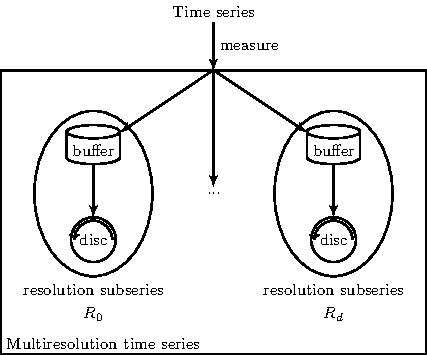
\includegraphics{fig_model_mtsdb.pdf}
  \caption{Architecture of \acro{MTSMS} model}
  \label{fig:model:mtsdb}
\end{figure}

The figure~\ref{fig:model:mtsdb} shows the architecture of a
\acro{MTSMS} for a single multiresolution time series.
%
In this way, the original time series gets stored in the resolution
subseries, each with a different time resolution and distinct
attribute aggregation policies. Discs are size bounded so they only
contain a fixed amount of measures. When a disc becomes full it
discards a measure. Thus, a multiresolution database is bounded in
size and the time series gets stored in a number of storage bounded
time subseries.

Regarding operations, the \acro{MTSMS} model requires two kind of
operators. Some operators should be devoted to set up the time
intervals between measures and to aggregate the attributes. Some other
operators should be dedicated to query the multiresolution schema and
to extract the time series data.

Following, we define the \acro{MTSMS} model structure and the
structural operators, the operations to query a multiresolution
schema, and the attribute aggregate functions.  Although schema
manipulation operations could be defined, in this paper we exclusively
focus on structure and data query operators.


\subsection{Structure}

A \emph{buffer} is a container for a time series. The aim of the
buffer is to regularise the time series using a constant resolution step
and an attribute aggregate function.  We name \emph{consolidation} to
this action of regularisation.  Note that the attribute aggregate
functions are defined in Section~\ref{sec:model:interpolador}.

\begin{definition}[Buffer]
  Let $S$ be a time series, let $\tau\in\cal{T}$ be the last
  consolidation time, let $\delta\in\cal{T}$ be the resolution step
  and let $f$ be an attribute aggregate function. We define a
  \emph{buffer} $B$ as the tuple $B=(S,\tau,\delta,f)$.
\end{definition}

An empty buffer is noted as $(\emptyset, t_0, \delta, f)$, that is an
empty time series, an initial consolidation time $t_0\in\cal{T}$, a
resolution step $\delta$ and a function $f$.  Given a buffer all the
consolidation time instants can be determined as $\tau_n=t+n\delta$
for all $n\in\N$.

Let $B=(S, \tau, \delta, f)$ be a buffer. The \emph{consolidation} of
$B$ is an operation that computes a new measure $m=f(S, \tau, \delta)$
summarising the data of $S$ comprised in the given interval.

A buffer has two main structural operations. The first one adds a
measure to the buffer and the second one consolidates the buffer.

Let $B=(S,\tau,\delta,f)$ be a buffer and let $m$ be a measure.  The
addition of $m$ to $B$, noted as $\addB(B,m)$, returns a new buffer
$\addB(B,m)=(S',\tau,\delta,f)$ where $S' = S \cup \{m\}$.

Let $B=(S,\tau,\delta,f)$ be a buffer. The consolidation of $B$, noted
as $\consB(B)$, returns a new buffer and a new measure $\consB(B)=(B',m')$
where $ B'= (S[\tau+\delta:+\infty], \tau+\delta,\delta,f)$ and $m' =
f(S,\tau,\delta)$. Note that after the consolidation, the
consolidated part of the time series can be removed from the buffer:
historic data is discarded.

The consolidation of a buffer is applied to the first non consolidated
time instant and the total consolidation is obtained by successive
application of the operator. 
%
This requires measures to be added by time order and to consolidate
the buffer when the time of some measure is bigger than the buffer's
next consolidation time.  
%
Let $B=(S,\tau,\delta,f)$ be a buffer and $m=\sup S$ the maximum
measure of $B$. We say that $B$ is consolidable if and only if $T(m)
\geq \tau+\delta$.

A \emph{disc} is a finite capacity container of measures. A time
series stored in a disc has its cardinal bounded. When the cardinal of
the time series is to overcome the limit, some measures need to be
discarded.

\begin{definition}[Disc]
  Let $k\in\N$ and $S$, $|S|\leq k$, be a time series. We define a
  \emph{disc} $D$ as the tuple $D=(S,k)$.
\end{definition}

An empty disc is noted as $(\emptyset,k)$. It is the tuple of an
empty time series and a bound $k$.

The main operation on a disc is to add a measure while keeping under
control the cardinal of the times series. Let $D=(S,k)$ be a disc and
let $m$ be a measure.  The addition of $m$ to $D$, written as
$\addD(D,m)$, is a new disc $\addD(D,m)=(S',k)$ where
%
\[
S' = \begin{cases}
  S\cup\{m\}                 & \text{if } |S|<k  \\
  (S-\{\min S\}) \cup \{m\} & \text{otherwise}
\end{cases}  
\]

A \emph{resolution subseries} is a structure that regularises and
aggregates a time series. It is composed of a buffer, which contains
the time series to be regularised, and a disc, which contains
the regularised time series.


\begin{definition}[Resolution subseries]
  Let $B$ be a buffer and let $D$ be a disc.  We define a
  \emph{resolution subseries} $R$ as the tuple $R=(B,D)$.  
\end{definition}
 
The operators of a resolution subseries extend the buffer and disc
ones. Let $R=(B,D)$ be a resolution subseries and let $m$ be a
measure.  The addition of $m$ to $R$, noted as $\addR(R,m)$, is a new
resolution subseries $\addR(R,m)=(B',D)$ where $B'= \addB(B,m)$ is the
addition of the measure to the buffer.  The consolidation of $R$,
noted as $\consR(R)$, is a new resolution subseries
$\consR(R)=(B',D')$ where $(B',m') = \consB(B)$ is the consolidation
of the buffer and $D'= \addD(D,m')$ is the addition of the
consolidated measure to the disc. A resolution subseries is
consolidable only when its buffer is consolidable.

A \emph{multiresolution time series} is a set of resolution subseries
referred to the same time series. We store a time series regularised
with distinct resolutions across the resolution subseries, as
previously shown in Figure~\ref{fig:model:mtsdb}.

\begin{definition}[Multiresolution time series]
  Let $M=\{R_0, \dots, R_k\}$ be a finite set of resolution
  subseries. Then $M$ is a \emph{multiresolution time series}.
\end{definition}

Therefore, to define a multiresolution time series we must define the
number of resolution subseries and its corresponding parameters
$(\delta,\tau,f,k)$.  Usually there are no repeated pairs of
$(\delta,f)$ parameters among a multiresolution series, so they act as
key attributes.

The operators of a multiresolution time series apply to every
resolution subseries contained. Let $M=\{R_0,\allowbreak
\dots,\allowbreak R_k\}$ be a multiresolution time series and let $m$
be a measure.
%
The addition of a measure to every resolution subseries, noted as
$\addM(M,m)$, is a new multiresolution time series $\addM(M,m)=\{R'_0,
\dots,\allowbreak R'_k\}$ where $R'_i=\addR(R_i,m)$. The consolidation
of all resolution subseries, noted as $\consM(M)$ is a new
multiresolution time series $\consM(M)=\{R'_0,\allowbreak
\dots,\allowbreak R'_k\}$ where
\[R'_i=
\begin{cases}
\consR(R_i) & \text{if } R_i \text{ consolidable}\\
 R_i & \text{otherwise}
\end{cases}
\]

% The multiresolution consolidation operation should be applied
% regularly based on a consolidation clock. When the measure ordered
% addition approach is taken as explained in the buffer's consolidation,
% then there is no need for a clock in a \acro{MTSMS}. The consolidation
% clock is induced by the measure's addition and then it is only
% necessary to check the multiresolution consolidation operation on new
% additions. However, there could be other approaches where the
% consolidation clock was given by an external clock or external
% events. Then the consolidable definitions would depend on this
% external clock.





\subsection{Queries}

There are two basic time series queries for a \acro{MTSMS}: (i) to
extract a time subseries from a resolution subseries or (ii) to query
for a total time series from all consolidated data.

% Aquesta sembla una consulta una mica circumstancial i menor ...
Let $M$ be a multiresolution time series and let $(\delta,f)$ be a
pair of key attributes.  The first query, denoted as
$\seriedisc(M,\delta,f)$, is a time series such that $\exists (B,D)
\in M: B=(S,\tau,\delta,f) \wedge D=(\seriedisc(M,\delta,f), k) $
where $S,\tau,k$ are bound variables.  Note that we
assume there are no repeated $(\delta,f)$ pairs in $M$.

Let $M=\{R_0,\dots,R_k\}$ be a multiresolution time series and let
$S_0,\dots,S_k$ the time series corresponding to the resolution
subseries $R_0,\dots,R_k$. Assume that the attribute aggregation
functions of all $R_i$ are the same and the resolution steps of all
$R_i$ are distinct.
%
We note as $\totalseries(M)$, the time ordered concatenation of all
time subseries. Recall that $R||S$ is the concatenation for two time
series $R$ and $S$, which has been defined in
Section~\ref{sec:sequence}. Assume that $i_0,\dots,i_k$ is a
permutation of $[0,k]$ such that $\delta_{i_0} < \delta_{i_1} < \cdots
< \delta_{i_k}$ being $\delta_i$ the resolution step of the resolution
subseries $R_i$. Then, $\totalseries(M) = S_{i_0} || S_{i_1} || \cdots
|| S_{i_k}$.
%
TotalSeries obtains the better possible resolution.

From these aforementioned basic time series queries, more elaborated
queries can be applied to \acro{MTSMS} by using \acro{TSMS}
operations. For example, let $L$ and $M$ be two multiresolution time
series, we can compute the sum of both as $\totalseries(L) +
\totalseries(M)$. Recall that $R+S$ is the sum of the values of two
time series $R$ and $S$, which has been defined in
Section~\ref{sec:set} as a binary computational operator.


\subsection{Attribute aggregate function}
\label{sec:model:interpolador}

Attribute aggregate functions are a specific case of \acro{TSMS}
aggregate operations used to summarise time series data while
consolidating a buffer.
%
% Let $S$ be a time series and let $[x,v]$ be a
% time interval. An attribute aggregate function $f$ calculates a new
% measure $m=f(S,[x,v])$. Then, this resulting measure $m$ is interpreted to
% summarise the measures of $S$ for the consolidation interval $[x,v]$.

Let $S$ be a time series, let $\delta$ be a resolution step and let
$\tau$ be a consolidation time.  An attribute aggregate function $f$
calculates a new measure $m=f(S,\tau,\delta)$. From $\tau$ and
$\delta$, we obtain the time interval $[\tau:\tau+\delta]$.  Then, the
resulting measure $m$ is interpreted to summarise the measures of $S$
for the time interval $[\tau:\tau+\delta]$.



% \[
% f : S=\{m_0,\ldots,m_k\} \times I=[t_i,t_j] \mapsto m'
% \]
% \[
% f: \cal{P}(\cal{T}\times\cal{V}) \times (\cal{T}\times\cal{T}) \rightarrow \cal{T}\times\cal{V}
% \]

An attribute aggregation function follows this general schema. First,
it obtains a time subseries $S'$ according to the consolidating
interval using a slice operator. For example, $S' =
S[\tau:\tau+\delta]$. Second, it applies a \acro{TSMS} aggregation
function on this time subseries to obtain $m$. For instance, $m =
\agg(S',n, g)$, being $g$ an aggregation function and $n$ an initial
measure, as defined in Section~\ref{sec:set}.

Many different attribute aggregate functions can be used in order to
summarise a time series, for example it is possible to calculate an
statistic indicator of the time series such as the average or a more
complex digital signal processing operation as proposed
by~\cite{zhang11}. Furthermore, the representation of a time series
and some of its pathologies can be considered during the aggregation
process.

Given the diversity of attribute aggregate functions, no global
assumptions can be made about them. Each user should decide which
combination of aggregation and representation fits better to the
measured phenomena.  Therefore, the \acro{MTSMS} model must have a
generic design that allows the users to define their own aggregate
functions.

In what follows we will give some examples of usual attribute
aggregation functions. These functions compute a new measure given a
set of known measures. Then, an attribute aggregation function should
compute a new time and a new value from the set known measures.
%
% For the rest of this Section we will write $m=f(S,[x,v])$ be the
% resulting measure of an attribute aggregation function $f$ applied to
% a time series $S$ for a time interval $[x,v]$.

% Sobre el calcul del nou temps

The attribute aggregation functions generally return measures that
match the buffer consolidating times. Assume, for instance, that $f$
is an attribute aggregation function and let $m=f(S,\tau,\delta)$.
Then, the time of $m$ is usually computed as $T(m)=\tau+\delta$.
%
However, in some cases it is preferred that $T(m)$ do not match the
buffer consolidating times.
%
For instance, the resulting measure can be aggregated from a time
subseries $S'$ using an open interval $S'=S(\tau:\tau+\delta)$, a
closed interval $S'=S[\tau:\tau+\delta]$, or other combinations like
$S'=S(\tau-d:\tau+\delta-d]$, where $d$ is a time duration that delays the
consolidation to $T(m)=\tau+\delta-d$.
%
This time offset can also be variable. For example, an aggregate
function that returns the first measure of the interval
$m=\min(S[\tau:\tau+\delta))$, then the resulting time fulfils that
$\tau\leq T(m) < \tau+\delta$.

% Sobre el calcul del nou valor
Assume that $f$ is an attribute aggregation function and let
$m=f(S,\tau,\delta)$.  An attribute aggregation function $f$ should
compute the value of $m$.
%
Next there are some examples that illustrate how to compute $V(m)$
based on the temporal function time series operators. 
That is, the time series aggregated is interpreted by the temporal
representation function $S(t)^r$ as has been described in
Section~\ref{sec:model:tfunc}. 
%
In these example functions we leave the time series representation $r$
uninstantiated.

\begin{itemize}
\item The \emph{maximum} computes $V(m)$ as $V(m) =
  \max\limits_{\forall t \in [\tau:\tau+\delta]} S(t)^r$. It
  summarises $S$ with the maximum of the measure values in the
  interval $[\tau:\tau+\delta]$.
\item The \emph{last} computes $V(m)$ as $V(m) = S(\tau+\delta)^r$. It
  summarises $S$ with the value at $\tau+\delta$ time instant.
\item The \emph{mean} computes $V(m)$ as $V(m) = \frac{1}{\delta}
  \int\limits_{\tau}^{\tau+\delta} S(t)^r dt$. It summarises $S$ with
  the mean of the function in the interval $[\tau:\tau+\delta]$.
\end{itemize}

The time series representation in previous examples can be
instantiated in several ways. In what follows we exemplify this
instantiating $r$ as \dd{} and \zohe{}.

Dirac delta attribute aggregation functions interpret the resulting
time as centered on the interval $T(m)=\frac{2\tau+\delta}{2}$. The
resulting value $V(m)$ depends on the attribute, let
$S'=S[\tau:\tau+\delta]^\dd$ be the selection of measures by Dirac
delta temporal interval. Then,
\begin{itemize}
\item The $maximum^\dd$ is such that $V(m) =
  \max\big(0,\max\limits_{\forall n \in S'} V(n)\big)$.
\item The $last^\dd$ is such that $V(m) = V(\max S')$.
\item The $mean^\dd$ is such that $V(m) = \frac{1}{\delta}
  \sum\limits_{\forall n \in S'} V(n)$. Note that for the Dirac
  delta function $\int\dd(t)dt=1$.
\end{itemize}

Note that $\sum\limits_{\forall n \in S'} V(n)$ is a sum of values
that could be implemented as $\agg(S',(0,0),g)$ where
$g(m,n)=(0,V(m)+V(n)$, as shown in
Example~\ref{ex:computational-operators}.

\zohe{} attribute aggregation functions interpret the resulting time
as the right limit of the interval $T(m)=\tau+\delta$. The resulting
value $V(m)$ depends on the attribute, let
$S'=S[\tau:\tau+\delta]^\zohe{}$ be the selection of measures by
\zohe{} temporal interval. Then,

\begin{itemize}
\item The $\maxz$ is such that $V(m) = \max\limits_{\forall n \in S'}
  V(n)$.
\item The $last^\zohe{}$ is such that $V(m) = V(\max S')$.
\item The $\meanz$ is such that $V(m) = \frac{1}{\delta}
  \big[(T(o)-\tau)V(o) + \sum\limits_{\forall n\in R}( T(n)-
  T(\prev_S n) )V(n)\big]$ where $o=\min S'$ and $R= S' - \{o\}$.\todo{repassar}
\end{itemize}

\emph{RRDtool}, \cite{rrdtool}, uses an aggregation function similar
to $\meanz$ to summarise velocity counter data by keeping the area
below the original signal.

It is interesting to note that some attribute aggregation patterns are
very similar. For instance, the maximum and last attribute aggregation
schemes differ basically on the interval selection operation. However,
other patterns have a more elaborated interpretation depending on the
actual representation used. This is the case of $\meanz$ and $mean^\dd$.


\begin{example}\label{ex:model:smultiresolution} 
  We define a multiresolution schema for a time series, we consolidate
  the database and we query its data.  Let $S = \{
  (1,6),(5,2),\allowbreak (8,5),\allowbreak (10,0),\allowbreak
  (14,1),\allowbreak (19,6),\allowbreak (22,11),\allowbreak
  (26,6),(29,0) \}$ be a time series and let $M=\{R_0,R_1\}$ be a
  multiresolution time series where each resolution parameters are
  $\tau_0=0$ , $\delta_0=5$, $f_0 =\meanz$, $k_0=4$ and $\tau_1=0$,
  $\delta_1=10$, $f_1 =\maxz$, $k_1=2$. Therefore $R_0$ will be
  consolidated at time instants 5, 10, 15, 20, 25, 30\dots and $R_1$
  at 10, 20, 30\dots

  All measures of $S$ are added to $M$
  and then it is consolidated until it is no more consolidable. As
  $T(\max S)=29$, the last consolidation times are $\tau_0=25$ and
  $\tau_1=20$, so we call $M_{29}$ to the multiresolution time series
  at this state.

  Then, the two time subseries consolidated are obtained by querying
  $\seriedisc(M_{29},5,\allowbreak \meanz)=\{\allowbreak
  (10,3),\allowbreak (15,\allowbreak 2),\allowbreak (20,7),\allowbreak
  (25,8)\}$ and $\seriedisc(M_{29},\allowbreak 10,\allowbreak \maxz)
  =\allowbreak \{ \allowbreak (10,6),\allowbreak (20,11)\}$. Regarding
  buffers, let $S_0$ and $S_1$ be the $M_{29}$ buffer's time series,
  note that $S_0= \{\allowbreak (26,6),\allowbreak (29,0)\allowbreak
  \}$ and $S_1=\{\allowbreak (22,11),\allowbreak (26,6),(29,0)\}$.

  In this particular example,
  $ \totalseries(M_{29}) = \seriedisc(M_{29},\allowbreak 5,\meanz)$ as $R_0$ has
  twice the resolution than $R_1$ and $k_0$ is bigger than $k_1$. 
\end{example}



%%% Local Variables:
%%% TeX-master: "main"
%%% ispell-local-dictionary: "british"
%%% End:

% LocalWords:  genericity multiresolution subseries consolidable

% LocalWords:  pathologies MTSMS TSMS cardinality multivalued infimum
% LocalWords:  multivalues supremum tuple affinely projectively MTSDB
%  LocalWords:  semitemporal piecewise TotalSeries RRDtool
